\documentclass[10pt,journal,compsoc]{IEEEtran}
%
% If IEEEtran.cls has not been installed into the LaTeX system files,
% manually specify the path to it like:
% \documentclass[10pt,journal,compsoc]{../sty/IEEEtran}





% Some very useful LaTeX packages include:
% (uncomment the ones you want to load)


% *** MISC UTILITY PACKAGES ***
%
%\usepackage{ifpdf}
% Heiko Oberdiek's ifpdf.sty is very useful if you need conditional
% compilation based on whether the output is pdf or dvi.
% usage:
% \ifpdf
%   % pdf code
% \else
%   % dvi code
% \fi
% The latest version of ifpdf.sty can be obtained from:
% http://www.ctan.org/pkg/ifpdf
% Also, note that IEEEtran.cls V1.7 and later provides a builtin
% \ifCLASSINFOpdf conditional that works the same way.
% When switching from latex to pdflatex and vice-versa, the compiler may
% have to be run twice to clear warning/error messages.






% *** CITATION PACKAGES ***
%
\ifCLASSOPTIONcompsoc
  % IEEE Computer Society needs nocompress option
  % requires cite.sty v4.0 or later (November 2003)
  \usepackage[nocompress]{cite}
\else
  % normal IEEE
  \usepackage{cite}
\fi
% cite.sty was written by Donald Arseneau
% V1.6 and later of IEEEtran pre-defines the format of the cite.sty package
% \cite{} output to follow that of the IEEE. Loading the cite package will
% result in citation numbers being automatically sorted and properly
% "compressed/ranged". e.g., [1], [9], [2], [7], [5], [6] without using
% cite.sty will become [1], [2], [5]--[7], [9] using cite.sty. cite.sty's
% \cite will automatically add leading space, if needed. Use cite.sty's
% noadjust option (cite.sty V3.8 and later) if you want to turn this off
% such as if a citation ever needs to be enclosed in parenthesis.
% cite.sty is already installed on most LaTeX systems. Be sure and use
% version 5.0 (2009-03-20) and later if using hyperref.sty.
% The latest version can be obtained at:
% http://www.ctan.org/pkg/cite
% The documentation is contained in the cite.sty file itself.
%
% Note that some packages require special options to format as the Computer
% Society requires. In particular, Computer Society  papers do not use
% compressed citation ranges as is done in typical IEEE papers
% (e.g., [1]-[4]). Instead, they list every citation separately in order
% (e.g., [1], [2], [3], [4]). To get the latter we need to load the cite
% package with the nocompress option which is supported by cite.sty v4.0
% and later. Note also the use of a CLASSOPTION conditional provided by
% IEEEtran.cls V1.7 and later.





% *** GRAPHICS RELATED PACKAGES ***
%
\ifCLASSINFOpdf
  % \usepackage[pdftex]{graphicx}
  % declare the path(s) where your graphic files are
  % \graphicspath{{../pdf/}{../jpeg/}}
  % and their extensions so you won't have to specify these with
  % every instance of \includegraphics
  % \DeclareGraphicsExtensions{.pdf,.jpeg,.png}
\else
  % or other class option (dvipsone, dvipdf, if not using dvips). graphicx
  % will default to the driver specified in the system graphics.cfg if no
  % driver is specified.
  % \usepackage[dvips]{graphicx}
  % declare the path(s) where your graphic files are
  % \graphicspath{{../eps/}}
  % and their extensions so you won't have to specify these with
  % every instance of \includegraphics
  % \DeclareGraphicsExtensions{.eps}
\fi
% graphicx was written by David Carlisle and Sebastian Rahtz. It is
% required if you want graphics, photos, etc. graphicx.sty is already
% installed on most LaTeX systems. The latest version and documentation
% can be obtained at: 
% http://www.ctan.org/pkg/graphicx
% Another good source of documentation is "Using Imported Graphics in
% LaTeX2e" by Keith Reckdahl which can be found at:
% http://www.ctan.org/pkg/epslatex
%
% latex, and pdflatex in dvi mode, support graphics in encapsulated
% postscript (.eps) format. pdflatex in pdf mode supports graphics
% in .pdf, .jpeg, .png and .mps (metapost) formats. Users should ensure
% that all non-photo figures use a vector format (.eps, .pdf, .mps) and
% not a bitmapped formats (.jpeg, .png). The IEEE frowns on bitmapped formats
% which can result in "jaggedy"/blurry rendering of lines and letters as
% well as large increases in file sizes.
%
% You can find documentation about the pdfTeX application at:
% http://www.tug.org/applications/pdftex



\usepackage{amsmath,amsfonts,amssymb}
\usepackage{algorithmic}
\usepackage{algorithm}
\usepackage{array}
\usepackage[caption=false,font=normalsize,labelfont=sf,textfont=sf]{subfig}
\usepackage{textcomp}
\usepackage{stfloats}
\usepackage{url}
\usepackage{verbatim}
\usepackage{graphicx}
\usepackage{cite}
%%%
\usepackage{xcolor}
\usepackage{tikz}

\newtheorem{theorem}{Theorem}
\newtheorem{lemma}{Lemma}
\newtheorem{remark}{Remark}
\newtheorem{assume}{Assumption}
\newtheorem{define}{Definition}

\begin{document}
\title{Randomized Matrix Weighted Consensus}
\author{Nhat-Minh Le-Phan,~Minh Hoang Trinh$^{\ast}$,~\IEEEmembership{Member,~IEEE},~Phuoc Doan Nguyen
        % <-this % stops a space
\IEEEcompsocitemizethanks{\IEEEcompsocthanksitem The authors are with the Department of Automation Engineering, School of Electrical and Electronic Engineering, Hanoi University of Science and Technology (HUST), Hanoi, Vietnam. N.M Le-Phan is also with Navigation, Guidance and Control Technologies Center, Viettel Aerospace Institute, Hanoi, Vietnam. E-mails: minh.lpn221013m@sis.hust.edu.vn; minh.trinh@ieee.org; phuoc.nguyendoan@hust.edu.vn. Corresponding author: M.~H.~Trinh.\protect}
\thanks{Manuscript received \ldots}
}


\IEEEtitleabstractindextext{%
\begin{abstract}
In this paper, a randomized gossip-type matrix-weighted consensus algorithm is proposed for both leaderless and leader-follower topologies. Under some mild assumptions, the proposed pairwise asynchronous update algorithm achieves a consensus in expectation. Moreover, the probability distribution, the weighting matrices, and the updating step size jointly determine the upper bound of the $\epsilon$-convergence time of the algorithm. Furthermore, we apply the proposed algorithm to the bearing-based network localization problem. The theoretical result is supported by several numerical examples.
\end{abstract}

% Note that keywords are not normally used for peerreview papers.
\begin{IEEEkeywords}
Matrix-weighted consensus, 	multi-agent systems, gossip algorithms, randomized algorithms. 
\end{IEEEkeywords}}


% make the title area
\maketitle

% To allow for easy dual compilation without having to reenter the
% abstract/keywords data, the \IEEEtitleabstractindextext text will
% not be used in maketitle, but will appear (i.e., to be "transported")
% here as \IEEEdisplaynontitleabstractindextext when the compsoc 
% or transmag modes are not selected <OR> if conference mode is selected 
% - because all conference papers position the abstract like regular
% papers do.
\IEEEdisplaynontitleabstractindextext
% \IEEEdisplaynontitleabstractindextext has no effect when using
% compsoc or transmag under a non-conference mode.

% For peer review papers, you can put extra information on the cover
% page as needed:
% \ifCLASSOPTIONpeerreview
% \begin{center} \bfseries EDICS Category: 3-BBND \end{center}
% \fi
%
% For peerreview papers, this IEEEtran command inserts a page break and
% creates the second title. It will be ignored for other modes.
\IEEEpeerreviewmaketitle



\IEEEraisesectionheading{\section{Introduction}\label{sec:introduction}}
% Computer Society journal (but not conference!) papers do something unusual
% with the very first section heading (almost always called "Introduction").
% They place it ABOVE the main text! IEEEtran.cls does not automatically do
% this for you, but you can achieve this effect with the provided
% \IEEEraisesectionheading{} command. Note the need to keep any \label that
% is to refer to the section immediately after \section in the above as
% \IEEEraisesectionheading puts \section within a raised box.


% The very first letter is a 2 line initial drop letter followed
% by the rest of the first word in caps (small caps for compsoc).
% 
% form to use if the first word consists of a single letter:
% \IEEEPARstart{A}{demo} file is ....
% 
% form to use if you need the single drop letter followed by
% normal text (unknown if ever used by the IEEE):
% \IEEEPARstart{A}{}demo file is ....
% 
% Some journals put the first two words in caps:
% \IEEEPARstart{T}{his demo} file is ....
% 
% Here we have the typical use of a "T" for an initial drop letter
% and "HIS" in caps to complete the first word.
%\section{Introduction}
\IEEEPARstart{I}{n} recent years, dynamics on complex networks has received a considered amount of research attention. Particularly, consensus algorithms have been shown to be essential for various applications \cite{Olfati2007consensuspieee} such as formation control, network localization, distributed estimation, synchronization, and social networks, \ldots

In a networked system, the dynamics of each agent in the system are often described by a vector of more than one state variable, and there may exist cross-layer couplings between these state variables. The authors in \cite{THM2018} proposed a matrix-weighted consensus algorithm, in which each pair-wise interaction between neighboring agents is associated with a symmetric nonnegative matrix weight. The matrix-weighted network, thus, provides a model for studying dynamics on a simplified multi-layer network. Corresponding to a matrix-weighted network system, one may define a matrix-weighted graph and its algebraic structure. Unlike scalar weighted graphs, connectedness of the network structure does not guarantee all agents to asymptotically achieve a common value under the matrix-weighted consensus algorithm. Algebraic and algorithms to determine whether the system would achieve consensus or clustering behaviors were considered in \cite{THM2018,Kwon2020matrix,Barooah2006graph,Pan2020controllability,Nguyen2022MCA}. Applications of the matrix-weighted consensus algorithm can be found in modelling multildimensional opinion dynamics \cite{Ahn2020opinion,Pan2018bipartite}, formation control and network localization \cite{bearingzhao,zhao2016aut,Barooah2006graph}, and the synchronization of multi-dimensional coupled mechanical and electrical systems \cite{Tuna2016aut,Tuna2019synchronization,Li2020synchronization}. 

It is noteworthy that most existing works on matrix-weighted consensus assumed that the agents update their states synchronously or following a deterministic update sequence. Continuous-time matrix-weighted consensus with switching graph topologies was studied in \cite{Pan2021consensus}. Discrete-time matrix-weighted consensus with fixed or switching topologies was studied in \cite{quoc2021}. Hybrid continuous-discrete time update algorithms were proposed in \cite{Miao2022TNSE,Miao2022consensus}.

{The randomized consensus algorithms, which refer to a family of consensus algorithms in which the edges between agents are randomly selected according to some stochastic model for every discrete instant, have received a lot of attention in the literature \cite{FB-LNS}. These algorithms, with their immense simplicity and reliability, have been successfully implemented for many applications in the next generation of networks, such as social networks, sensor networks, and peer-to-peer networks,... The randomized gossip algorithm, which is proposed in \cite{boyd2006}, was a significant step toward solving the average consensus problem in a randomized manner. In this algorithm, a pair of agents $i$ and $j$ are said to "gossip" at a discrete time instant $k$ if they set their next values as the average of their current ones. The random aspect is clarified by aligning each agent with a clock that "ticks"
are distributed as a rate 1 Poisson process. In other words, at each time slot, there will be one agent $i$ who wakes up with a probability $\frac{1}{n}$, and it will choose another agent $j$ with a probability ${\rm P}_{ij}$ (conditional to $i$ being selected) to gossip.} Many approaches have been proposed based on \cite{boyd2006} to enhance its convergence speed as well as robustness, see for example, \cite{5625615,TIT2010,1238221} on geographic gossip; \cite{HE20118718,7887729,LABAHN1994235} on periodic gossiping; \cite{7581065,4787122} on broadcast gossip; \cite{8946047} on reduce the probability of selecting duplicate nodes,\dots However, these studies only cover the situation when the connecting weights between agents are scalar, i.e., they do not have the ability to deal with the coupling mechanism for agents with multi-dimensional state vectors.

In this paper, we firstly study the dynamics of a matrix-weighted graph under the pair-wise gossiping update protocol proposed in \cite{boyd2006}. To the best of our knowledge, this is the first work considering randomized and asynchronous update approaches for matrix-weighted multi-agent systems. As a result, the randomized algorithm in this paper extends the applicability and practicality of the matrix-weighted consensus to various aforementioned applications. Secondly, to guarantee the consensus, \cite{boyd2006,5340530} require constraints regarding the first two moments of the updating matrix, which are mostly related to the connectivity of the network. For achieving a randomized matrix-weighted consensus, the sufficient consensus condition in this work are jointly determined by both the eigenvalues of the expected graph Laplacian and the local matrix weights of each agent. Lastly, the proposed algorithm is then applied to the bearing-based network localization in sensor networks.

The remainder of this paper is organized as follows. In Section \ref{sec:prel}, we introduce the preliminaries and problem formulation. Our works on randomized matrix-weighted consensus algorithms for leaderless and leader-follower topologies  are covered in Section \ref{sec:leaderless} and Section \ref{sec:leader-follower}, respectively. A randomized bearing-based network localization algorithm is presented in Section~\ref{section: NL}. Numerical simulation are provided in Section \ref{section: simulation} to support the theoretical results. Finally, we summarize the paper and outline directions for future research in Section \ref{sec:conclusion}.

\section{Preliminaries and problem formulation}
\label{sec:prel}
\subsection{Matrix-weighted graphs and the expected graphs}
A directed matrix-weighted graph is denoted by $ \mathcal{G}=(V,E,A)$, where, $V=\left\{ 1,2,...,n\right\}$ is the vertex set (agents), $E\subseteq V\times V$ is the edge set, and 
$A=\{ \mathbf{A}_{ij} \in \mathbb{R}^{d \times d}|~(i,j) \in E\}$ denotes the set of matrix weights. $d \geq 1$ is the dimension of each agent's state vector. When $d = 1$, $\mathcal{G}$ reduces to a scalar graph. The interactions between any two agents in $\mathcal{G}$ are captured by the corresponding matrix weights: if $i$ can communicate with $j$, there is a symmetric positive definite/positive semi-definite matrix weight $\mathbf{A}_{ij}=\mathbf{A}_{ij}^\top\geq 0$; and if $i$ does not have a communication link with $j$, then  $\mathbf{A}_{ij}$ is the zero matrix. We call an edge $(i,j)$ positive definite (resp., positive semi-definite) if the related matrix weight is positive definite (resp., positive semi-definite). Let $\mathbf{D}_{i}= \sum_{j \in V} \mathbf{A}_{ij}$ be the matrix-degree of vertex $i$, and $\mathbf{D} = \text{blkdiag}(\mathbf{D}_{1}, \ldots,\mathbf{D}_{n})$ denote \emph{degree matrix} of $\mathcal{G}$. The \emph{matrix-weighted Laplacian} is then defined as $\mathbf{L} = \mathbf{D} - \mathbf{A} \in \mathbb{R}^{nd \times nd}$. 

\begin{figure}
    \centering
    \includegraphics[width=\linewidth]{graphSymmetrization.png}
    \caption{A directed matrix-weighted graph $\mathcal{G}$ and its corresponding expected graph $\mathcal{G}^{\rm M}$.}
    \label{fig:graphSymmetrization}
\end{figure}
For each edge in $E$, we associate a corresponding number ${\rm P}_{ij}\in [0,1]$, which is the probability that a vertex $j \in V$ is chosen by vertex $i$ for updating information, $\sum_{j=1}^n{\rm P}_{ij}=1$. Defining $\mathbf{M}_{ij}=\frac{1}{n}(\mathbf{A}_{ij} {\rm P}_{ij}+\mathbf{A}_{ji} {\rm 
 P}_{ji})$ as the \emph{expected matrix weight} between two vertices $i$ and $j$, it is obvious that $\mathbf{M}_{ij}=\mathbf{M}_{ji}=\mathbf{M}_{ij}^{\top} \geq 0$. Thus, the digraph $\mathcal{G}$ induces a corresponding \emph{undirected} matrix-weighted graph $\mathcal{G}^{\rm M}=(V,E^{\rm M},A^{\rm M})$, where $E^{\rm M}=\{(i,j)|~\mathbf{M}_{ij} \neq 0)\}$ and $A^{\rm M}=\{ \mathbf{M}_{ij}\}_{(i,j)\in E^{\rm M}}$. Figure~\ref{fig:graphSymmetrization} depicts a graph $\mathcal{G}$ and its expected graph $\mathcal{G}^{\rm M}$. 
 
 Let $\mathbf{A}^{\rm M}=[\mathbf{M}_{ij}]$, $\mathbf{D}^{\rm M}$, and $\mathbf{L}^{\rm M} = \mathbf{D}^{\rm M}-\mathbf{A}^{\rm M} \in \mathbb{R}^{nd \times nd}$ correspondingly the \emph{expected adjacency matrix}, the \emph{expected degree matrix}, and the \emph{expected Laplacian matrix} of $\mathcal{G}$.\footnote{or, they can be simply refered to as the matrix-weighted adjacency/degree/Laplacian matrix of $\mathcal{G}^{\rm M}$.} All existing results on undirected matrix-weighted graphs can be used for studying the expected graph $\mathcal{G}^{\rm}$. An positive path $\mathcal{P}=i_1,i_2,...,i_l \in \mathcal{G}^{\rm M}$ is a sequence of non-repeating edges in $V$ such that $\mathbf{M}_{i_{k}i_{k+1}} > 0, k=1,...,l-1$. 
A positive spanning tree $\mathcal{T}^{\rm M}$ is a graph consisting of $n$ vertices and $(n-1)$ edges in $\mathcal{G}^{\rm M}$ so that there exists a unique positive path between any pair of vertices in $\mathcal{T}^{\rm M}$.
 
\begin{lemma}\label{nullspace}
\emph{\cite{THM2018}}
The expected Laplacian matrix $\mathbf{L}^{\rm M}$ is symmetric and positive semi-definite. Moreover, 
  ${\rm null}(\mathbf{L}^{\rm M}) = {\rm span}\{ {\rm range}(\mathbf{1}_n \otimes \mathbf{I}_d), \{ \mathbf{v}=[v_1^\top,\dots, v_n^\top]^\top \in \mathbb{R}^{nd}|~(v_j-v_j)\in {\rm null}(\mathbf{M}_{ij}), \forall (i,j) \in E \} \}$.
\end{lemma}
\subsection{Randomized distributed protocol}
In this section, we describe the basic protocol that will be used for the rest of this article, which can be found in \cite{ishii2010}. Consider the multiagent system from the previous section. The random manner is specified by the random process $\gamma(k)\in V$ where $k\in \mathbb{Z}_{+}$ is called time slot. At time slot $k$, $\gamma(k) = i$ indicates that agent $i$ wakes up, then it will choose another neighbor $j$ with a probability $P_{ij}$ to communicate, and both agents update their state values. $\gamma(k)$ is assumed to be i.i.d., and its probability distribution is given by
\begin{equation}\label{manner}
{\rm P}(\gamma(k)=i)=\frac{1}{n}, \forall k\in \mathbb{Z}_{+}.
\end{equation}
This means the distribution of agents choosing to wake up at any time slot is uniform. This protocol can be implemented distributively by giving each agent an independent clock that ``ticks'' (wakes the agent up) at the times of an identical stochastic process. For example, \cite{boyd2006} sets a clock that
``ticks'' are distributed as a rate 1 Poisson process for each agent. In this paper, we do not restrict to any particular stochastic process for the purpose of simplicity. Because time slots are the only instances when the value of each agent changes \cite{boyd2006}, we will utilize them as a new time axis in all of our results. The matrix-weighted consensus laws for both leaderless and leader-following topologies based on the discussed protocol will be introduced in the next section.
\begin{lemma}
\emph{(Markov inequality)} If a random variable X can only take non-negative values, then \cite{prob}:
   $${\rm P}(X>a) \leq \frac{{{\rm E}}[X]}{a}, \ \  \forall a >0,$$
where ${\rm E}[X]$ is the expectation of X.
\end{lemma}
\section{Randomized matrix weighted consensus with Leaderless topology}
\label{sec:leaderless}
In this section, we propose the randomized matrix-weighted consensus law with leaderless topology as follows
Consider a system consisting of $n$ agents whose interconnections between agents are $\mathbf{A}_{ij}\in\mathbb{R}^{d\times d}$. Each agent $i\in V$ stores its own local vector $\overline{x}_i \in \mathbb{R}^d$. When an agent $i$ wakes up at the $k^{\text{th}}$ time slot, it will contact a neighbor $j$ with a probability ${\rm P}_{ij}$ and both agents will update their current state vector as:
\begin{equation}\label{algorithm1}
    \begin{aligned}
    \overline{x}_i(k+1)&=\overline{x}_i(k)-\alpha_i \mathbf{A}_{ij}\big(\overline{x}_i(k)-\overline{x}_j(k)\big)\\
    \overline{x}_j(k+1)&=\overline{x}_j(k)-\alpha_j \mathbf{A}_{ij}\big(\overline{x}_j(k)-\overline{x}_i(k)\big)\\
    \end{aligned}
\end{equation}
where $\alpha_i > 0$ is updating step size of agent $i$, and will be designed later.
\begin{assume}\label{pii}
When an agent wakes up, it chooses another agent in the network to exchange information, that is, $P_{ii}=~ 0$ for all $i\in V$.
\end{assume}
Denote $\overline{\mathbf{x}}(k) = \text{vec}(\overline{\mathbf{x}}_i(k))$, (\ref{algorithm1}) can be rewritten as follow:
\begin{equation}\label{algorithm11}
    \overline{\mathbf{x}}(k+1)=W_{ij}\overline{\mathbf{x}}(k),
\end{equation}
where $W_{ij}$ is a block matrix: 
{\small
\begin{equation}\label{algorithm12}
W_{ij}=\begin{bmatrix}
    &\mathbf{I}_d        &\cdots     &\mathbf{0}            &\cdots    &\mathbf{0} &\cdots &\mathbf{0} \\
    &\vdots     &\ddots     &\vdots          &\ddots    &\vdots &\ddots &\vdots \\
    &\mathbf{0}       &\cdots  &\mathbf{I}_d-\alpha_i \mathbf{A}_{ij} &\cdots    &\alpha_i \mathbf{A}_{ij} &\cdots &\mathbf{0} \\
    &\vdots     &\ddots     &\vdots          &\ddots    &\vdots &\ddots &\vdots \\
    &\mathbf{0}      &\cdots  &\alpha_j \mathbf{A}_{ij} &\cdots    &\mathbf{I}_d-\alpha_j\mathbf{A}_{ij} &\cdots &\mathbf{0}  \\
    &\vdots     &\ddots     &\vdots          &\ddots    &\vdots &\ddots &\vdots \\
    &\mathbf{0}       &\cdots     &\mathbf{0}            &\cdots    &\mathbf{0} &\cdots &\mathbf{I}_d
\end{bmatrix}
\end{equation}}
in which $\mathbf{I}_d$ denotes the $d\times d$ identity matrix, $\mathbf{0}$ denotes the $d\times d$ zero matrix, $\mathbf{I}_d-\alpha_i \mathbf{A}_{ij}$ is the block entry of matrix $W_{ij}$ in the $({i(d-1)+1:id})^{\text{th}}$ rows
and $({i(d-1)+1:id})^{\text{th}}$ columns. Block $\mathbf{I}_d-\alpha_j \mathbf{A}_{ij}$ is in the $({j(d-1)+1:jd})^{\text{th}}$ rows
and $({j(d-1)+1:jd})^{\text{th}}$ columns of $W_{ij}$. Due to the symmetry of $\mathbf{A}_{ij}$, $W_{ij}$ is also symmetric.

At a random $k^{\text{th}}$ time slot, we can write:
\begin{equation}\label{algorithm13}
\overline{\mathbf{x}}(k+1)=W(k)\overline{\mathbf{x}}(k),
\end{equation}
where the random variable $W(k)$ is drawn i.i.d from some distribution on the set of possible values $W_{ij}$ \cite{boyd2006}. Note that the probability that $W(k)$ takes a specific value $W_{ij}$ is $\frac{1}{n}{\rm P}_{ij}$ (the probability that agent $i$ will wake up at $k^{\text{th}}$ time slot is $\frac{1}{n}$, and the probability that $j$ will be chosen by $i$ is ${\rm P}_{ij}$). The expectation of $W(k)$ is thus obtained as
\begin{equation}
    \begin{aligned}
        \overline{W}={\rm E}[W]=\sum_{i \in V}\sum_{j \in V} \frac{1}{n}{\rm P}_{ij} W_{ij}.
    \end{aligned}
\end{equation}
The block entries of $\overline{W}$ are determined as follow:
\begin{itemize}
    \item If $i=j$, then:
    \begin{align*}
        \overline{W}&(i,i)=\bigg(1-\frac{1}{n}\sum_{j\in V}({\rm P}_{ij}+{\rm P}_{ji})\bigg)\mathbf{I}_d \nonumber\\
        &+\frac{1}{n}\sum_{j \in V}\big({\rm P}_{ij}(\mathbf{I}_d-\alpha_i \mathbf{A}_{ij})+{\rm P}_{ji}(\mathbf{I}_d-\alpha_i \mathbf{A}_{ji})\big) \nonumber\\
        &\qquad= \mathbf{I}_d - \alpha_i\frac{1}{n}\sum_{j \in V}({\rm P}_{ij} \mathbf{A}_{ij}+{\rm P}_{ji} \mathbf{A}_{ji}) \nonumber\\
        &\qquad= \mathbf{I}_d-\alpha_i\sum_{j \in V}\mathbf{M}_{ij}.
    \end{align*}
    \item If $i \neq j$:
\begin{align*}
\overline{W}(i,j)&=\frac{\alpha_i}{n} %\sum_{j \in V}
({\rm P}_{ij} \mathbf{A}_{ij} + {\rm P}_{ji} \mathbf{A}_{ji}) =\alpha_i 
\mathbf{M}_{ij}.
\end{align*}
\end{itemize}
As a result, \eqref{algorithm13} can be rewritten as:
\begin{equation}\label{wbar}
\overline{W}=\mathbf{I}_{dn} - \mathbf{G}(\mathbf{D}^{\text{M}}-\mathbf{A}^\text{M}),
\end{equation}
where $\mathbf{G}=\text{blkdiag}\left\{\alpha_i\mathbf{I}_d\right\}_{i=1}^n$.
\subsection{Convergence in expectation}
The solution of (\ref{algorithm13}) can be easily obtained as:
\begin{equation}\label{sol}
\overline{\mathbf{x}}(k+1) = \underbrace{W(k)W(k-1)\dots W(0)}_{:=\phi(k)} \overline{\mathbf{x}}(0).
\end{equation}
In order to prove the convergence in expectation, we consider the mean of $\phi(k)$
\begin{equation}\label{mean}
    \begin{aligned}
        {\rm E}[\phi(k)]&={\rm E}[W(k)W(k-1)\dots W(0)] \\
        &={\rm E}[W(k)]{\rm E}[W(k-1)]\dots{\rm E}[W(0)]\\
        &=\overline{W}^{k+1}=\big(\mathbf{I}_{dn}-\mathbf{G}(\mathbf{D}^\text{M}-\mathbf{A}^\text{M})\big)^{k+1}.
    \end{aligned}
\end{equation}
Thhe spectral properties of $\overline{W}$  is stated in the following lemma, whose proof can be found in \cite{quoc2021}.
\begin{lemma}\label{stepsize}
Let the step sizes satisfy $\alpha_i < \frac{1}{\lVert \mathbf{D}^{{\rm M}}_{i} \rVert}$. The matrix $\overline{W}= \mathbf{I}_{dn}-\mathbf{G}(\mathbf{D}^{\rm M}-\mathbf{A}^{\rm M})$ satisfies the following properties:
\begin{itemize}
    \item All eigenvalues of $\overline{W}$ lie in the range $(-1,1]$ and the spectral radius is $\rho(\overline{W})=1$ with the corresponding eigenvectors that are $\mathbf{\textit{v}}\in {\rm null}(\mathbf{L}^{\rm M})$.
    \item The unity eigenvalue 1 of $\overline{W}$ is semi-simple, and $\overline{W}^{\infty}:=\lim_{k\to \infty} \overline{W}^{k}$ exists and is finite. 
\end{itemize}
\end{lemma}
Regarding the existence of $\overline{W}^{\infty}$, we have 
\begin{equation}
    \begin{aligned}
        \overline{W}^{\infty}&=(\mathbf{V}\mathbf{J}\mathbf{V}^{-1})^{\infty}=\mathbf{VJ^{\infty}V^{-1}}\\
        &=\mathbf{V}\text{blkdiag}(1,\dots,1,\mathbf{J}_{l_2}^{\infty},\dots,\mathbf{J}_{l_p}^{\infty})\mathbf{V}^{-1}\\
        &=\mathbf{V}\text{blkdiag}(1,\dots,1,0,\dots,0)\mathbf{V}^{-1}=\sum_{i=1}^{l_1}v_i u_i^{\top},
    \end{aligned}
\end{equation}
where $\mathbf{V}=[v_1,\dots,v_{dn}]$ and $\mathbf{V}^{-1}=[u_1,\dots,u_{dn}]^{\top}$ contain the left and right eigenvectors of $\overline{W}$, respectively. The Jordan form 
$\mathbf{J}=\text{blkdiag}(1,\dots,1,\mathbf{J}_{l_2},\dots,\mathbf{J}_{l_p}) \in \mathbb{R}^{dn\times dn}$ contains Jordan blocks $\mathbf{J}_{l_i},i=2,\ldots,p,$ corresponding to the eigenvalues $\lambda_i$ with magnitudes strictly smaller than 1. It follows that
\begin{align}
    \lim_{k\to \infty} {\rm E}[\bar{\mathbf{x}}(k)]= \left( \lim_{k\to \infty} \bar{W}^k \right) \bar{\mathbf{x}}(0) = \sum_{i=1}^{l_1}v_i u_i^{\top} \bar{\mathbf{x}}(0).
\end{align}
Combining with Lemma~\ref{nullspace}, we have the following theorem.

\begin{theorem}\label{conthm}
Select the step sizes to satisfy Lemma~\ref{stepsize}. For all $\mathbf{\overline{x}}(0)$, the solution $\mathbf{\overline{x}}(k)$ of \eqref{sol} converges in the expectation to $\mathbf{\overline{x}}^{*}=\mathbf{1}_n\otimes \big([{{u}}_1, {{u}}_2,\dots,{{u}}_d]^\top \mathbf{x}(0) \big)$, if and only if {\rm null}$(\mathbf{L}^{\rm M})=${\rm range}$(\mathbf{1}_n \otimes \mathbf{I}_d)$.
\end{theorem}
\begin{remark} \cite{THM2018} The existence of a positive spanning tree in $\mathcal{G}^{\rm M}$ is a sufficient condition for ${\rm null}(\mathbf{L}^{\rm M})={\rm range}(\mathbf{1}_n\otimes \mathbf{I}_d)$.
 \end{remark}
 \subsection{Randomized matrix weighted average consensus}
 When all agents choose the same updating step size $\alpha$, the matrix $\overline{W}$ becomes symmetric, and $\mathbf{V}^{\top}=\mathbf{V}^{-1}$. The following theorem yields
 \begin{theorem}\label{avconthm}
Suppose that all agents use the same step size $\alpha < \frac{1}{\max_{i\in V}\lVert \mathbf{D}^{\rm M}_{i} \rVert}$. For all $\mathbf{\overline{x}}(0)$, the solution $\mathbf{\overline{x}}(k)$ of (\ref{sol}) converges in expectation to the average vector $\mathbf{\overline{x}}^{*}= \mathbf{1}_n \otimes \hat{\mathbf{x}}$, where $\hat{\mathbf{x}}=\frac{1}{n}\big(\mathbf{1}_n^\top\otimes \mathbf{I}_d\big)\mathbf{\overline{x}}(0)$, if and only if {\rm null}$(\mathbf{L}^{\rm M})={\rm range}(\mathbf{1}_n\otimes \mathbf{I}_d)$.
\end{theorem}

Although we have shown that, if the graph $\mathcal{G}$ satisfies a mild assumption and the step size is  small enough, it is guaranteed that the agents reach the average consensus in expectation. However, we have not yet mentioned the convergence rate of these agents. The following section  will describe a method to quantify the average convergence rate of agents. It will be shown that the convergence rate of the agents is closely related to the second-largest amplitude eigenvalue of the matrix ${\rm E}[W(k)^\top W(k)]$. Inspired by \cite{boyd2006}, we first introduce our quantity of interest
\begin{define}
 \emph{($\epsilon$-consensus time)} For any $0<\epsilon<1$, the $\epsilon$-consensus time is defined as:
\begin{equation}
\begin{aligned}
    T(\epsilon)=\underset{\overline{\mathbf{x}}(0)}{\sup}\inf \bigg( k:{\rm P}\bigg(\frac{\lVert \mathbf{\overline{x}}(k)-\mathbf{1}_n\otimes \hat{\mathbf{\overline{x}}} \rVert}{\lVert \mathbf{\overline{x}}(0)-\mathbf{1}_n\otimes \hat{\mathbf{\overline{x}}} \rVert} \geq \epsilon\bigg)\leq \epsilon\bigg)
\end{aligned}
\end{equation}
\end{define}
Intuitively, $T({\epsilon})$ represents the number of clock ticks needed for the trajectory $\mathbf{\overline{x}}$ to reach the consensus value with a high probability. It is worth noting that $\epsilon$ measures both accuracy and success probability and is often set to $\frac{1}{n}$ \cite{TIT2010}. In this paper, we provide the upper bound formula for the proposed average consensus algorithm. Firstly, the convergence of the second moment will be proved.
\subsubsection{Convergence of the second moment}
Define the error vector $\mathbf{\overline{y}}(k)=\mathbf{\overline{x}}(k)-\mathbf{1}_n\otimes \hat{\mathbf{\overline{x}}}$, we have
\begin{equation}\label{y}
\begin{aligned}
    \mathbf{\overline{y}}(k+1)&= \mathbf{\overline{x}}(k+1)-\mathbf{1}_n\otimes \hat{\mathbf{\overline{x}}}\\
%    &=W(k)\mathbf{\overline{x}}(k)-\mathbf{1}_n\otimes \mathbf{I}_d\hat{\mathbf{\overline{x}}}\\
%    &=W(k)\mathbf{\overline{x}}(k)-(\mathbf{1}_n\otimes \mathbf{I}_d)\hat{\mathbf{\overline{x}}}\\    
    &=W(k)\mathbf{\overline{x}}(k)-W(k)(\mathbf{1}_n\otimes \mathbf{I}_d)\hat{\mathbf{\overline{x}}}\\  
%    &=W(k)\big(\mathbf{\overline{x}}(k)-(\mathbf{1}_n\otimes \mathbf{I}_d)\hat{\mathbf{\overline{x}}}\big)\\
%    &=W(k)\big(\mathbf{\overline{x}}(k)-\mathbf{1}_n\otimes \hat{\mathbf{\overline{x}}}\big)\\  
    &=W(k)\mathbf{\overline{y}}(k).
\end{aligned}
\end{equation}
Thus, $\mathbf{\overline{y}}(k)$ has the same linear system as $\mathbf{\overline{x}}(k)$. From \eqref{y}, we have the following equation \cite{boyd2006}
\begin{equation}\label{minh}
    \begin{aligned}
        {\rm E}[\mathbf{\overline{y}}(k+1)^{\top}\mathbf{\overline{y}}(k+1)|\mathbf{\overline{y}}(k)]
        = \mathbf{\overline{y}}(k)^{\top}{\rm E}[W(k)^{\top}W(k)]\mathbf{\overline{y}}(k)
    \end{aligned}
\end{equation}
Similar to $W(k)$, we can consider $W(k)^\top W(k)$ as a random variable which is drawn i.i.d from some distribution on the set of possible values $W_{ij}^\top W_{ij}$. Some properties of ${\rm E}[W(k)^\top W(k)]$ are provided by the following lemmas.
 \begin{lemma}\label{stepsizeav}
Let the step size for each agent satisfy $\alpha < \underset{i,j}{\min}(\frac{1}{\max\lVert \mathbf{D}^{\rm M}_{i} \rVert},\frac{1}{\max\lVert \mathbf{A}_{ij} \rVert})$, the following statements hold
\begin{enumerate}
    \item The set of all real symmetric matrices with eigenvalues in $[0,1]$ is convex. Every possible matrix $W_{ij}^\top W_{ij}$ is in this set.
    \item ${\rm E}[W(k)^\top W(k)]$ has a unity spectral radius, and its unity eigenvalues are semi-simple.
    \item $\mathbf{1}_n \otimes\mathbf{I}_d$ are 
only $d$ orthogonal right eigenvectors corresponding to the unity eigenvalue $\lambda=1$ of ${\rm E}[W(k)^\top W(k)]$ if and only if {\rm null}$(\mathbf{L}^{\rm M})= {\rm range}(\mathbf{1}_n\otimes \mathbf{I}_d)$.
\end{enumerate}
    
\emph{Proof:} See Appendix A.
\end{lemma}
Under the assumption null$(\mathbf{L}^{\text{M}})=\text{range}(\mathbf{1}_n\otimes \mathbf{I}_d)$ on our hand, $[v_1,\dots,v_d] =\mathbf{1}_n \otimes\mathbf{I}_d$ are 
only $d$ orthogonal right eigenvectors corresponding to the unity eigenvalue $\lambda=1$ of ${\rm E}[W(k)^\top W(k)]$. By reason of $\mathbf{\overline{y}}(k)\perp \text{span}\big( v_1,\dots,v_d \big)$, the Rayleigh-Ritz theorem states that
%\begin{equation}
\begin{align} \label{raritz}
\mathbf{\overline{y}}(k)^\top &{\rm E}[W(k)^\top W(k)] \mathbf{\overline{y}}(k) \nonumber\\
      &\leq \lambda_{d+1}({\rm E}[W(k)^\top W(k)]) \mathbf{\overline{y}}(k)^\top \mathbf{\overline{y}}(k)
\end{align}
%\end{equation}
where $\lambda_{d+1}<1$ is the second largest eigenvalue of ${\rm E}[W(k)^\top W(k)]$. After iterating (\ref{minh}) and (\ref{raritz}), we get:
\begin{equation}\label{raritz2}
    \begin{aligned}
      {\rm E}[\mathbf{\overline{y}}(k)^\top \mathbf{\overline{y}}(k)] \leq \lambda_{d+1}^{k}({\rm E}[W(k)^\top W(k)]) \mathbf{\overline{y}}(0)^\top \mathbf{\overline{y}}(0)
    \end{aligned}
\end{equation}
which also implies that the convergence of the second moment of the proposed algorithm. 

When the matrix weight $\mathbf{A}_{ij}$ is nonsymmetric in general, necessary and sufficient conditions can be obtained by applying the results proposed in \cite{boyd2006,1272421}, which are as follow
\begin{lemma}\label{iff}
 {The first and second moment of the solution of (\ref{algorithm11}) will converge in probability if and only if there exists a common stepsize $\alpha$ such that
\begin{enumerate}
    \item $\rho\big(\overline{W}-\frac{(\mathbf{1}_n\mathbf{1}_n^\top)\otimes\mathbf{I}_d}{n}\big)<1$,
    \item $\rho\big({\rm E}[W(k)\otimes W(k)]-\frac{(\mathbf{1}_{n^2}\mathbf{1}_{n^2}^\top)\otimes\mathbf{I}_{d^2}}{n^2}\big)<1$.
\end{enumerate}
}
\end{lemma}
{In Lemma \ref{iff}, the first constraint makes all agents reach the average consensus, whereas the second guarantees the convergence of the second moment. However, despite having explicit criteria for the convergence of the second moment, it is clearly seen that these requirements are not intuitive and quite hard to assess. Moreover, the symmetry of $\mathbf{A}_{ij}$ allows us to find interesting results of $\epsilon$-consensus time, which will be provided later.}
\subsubsection{Upper bound of the $\epsilon$-consensus time}
\begin{theorem}\label{upperbound1}
    Select a common step size for every agent such that $\alpha < \underset{i,j}{\min}(\frac{1}{\max\| \mathbf{D}^{\rm M}_{i} \|},\frac{1}{\max \| \mathbf{A}_{ij} \|})$. With an arbitrary initial  state vector $\mathbf{\overline{x}}(0)$, the solution $\mathbf{\overline{x}}(k)$ of \eqref{sol} converges in the expectation to the average vector $\mathbf{\overline{x}}^{*}=\bigg(\frac{1}{n} \mathbf{1}_n\mathbf{1}_n^\top \otimes \mathbf{I}_d \bigg)\mathbf{\overline{x}}(0)$ if and only if ${\rm null}(\mathbf{L}^{\rm M})={\rm range}(\mathbf{1}_n\otimes \mathbf{I}_d)$. Furthermore, the $\epsilon$-consensus time is upper bounded by a function of the second largest eigenvalue of ${\rm E}[W(k)^\top W(k)])$.
\end{theorem}
\emph{Proof:} Using Markov's inequality, we have:
\begin{align}
        {\rm P}\bigg(\frac{\lVert \mathbf{\overline{x}}(k)-\mathbf{1}_n\otimes \hat{\mathbf{\overline{x}}} \rVert}{\lVert \mathbf{\overline{x}}(0)-\mathbf{1}_n\otimes \hat{\mathbf{\overline{x}}} \rVert} & \geq \epsilon \bigg) 
        ={\rm P}\bigg(\frac{\mathbf{\overline{y}}(k)^\top \mathbf{\overline{y}}(k)}{\mathbf{\overline{y}}(0)^\top \mathbf{\overline{y}}(0)}\geq \epsilon^2\bigg) \nonumber\\
        &\leq\frac{\epsilon^{-2}{\rm E}[\mathbf{\overline{y}}(k)^\top \mathbf{\overline{y}}(k)]}{\mathbf{\overline{y}}(0)^\top \mathbf{\overline{y}}(0)} \nonumber\\
        &\leq \epsilon^{-2} \lambda_{d+1}^k \big( {\rm E}[\mathbf{\overline{W}}(k)^\top \mathbf{\overline{W}}(k)] \big).
\end{align}

As a result, for $k \geq K(\epsilon)=\frac{3{\log}(\epsilon^{-1})}{{\log}\lambda_{d+1}^{-1} \big( {\rm E}[\mathbf{\overline{W}}(k)^\top \mathbf{\overline{W}}(k)] \big)}$, there holds
$$\rm{P}\bigg(\frac{\lVert \mathbf{\overline{x}}(k)-\mathbf{1}_n\otimes \hat{\mathbf{\overline{x}}} \rVert}{\lVert \mathbf{\overline{x}}(0)-\mathbf{1}_n\otimes \hat{\mathbf{\overline{x}}} \rVert} \geq \epsilon \bigg) \leq \epsilon.$$ 
This implies $K(\epsilon)$ is the upper bound of the $\epsilon$-consensus time. 

\section{Randomized matrix weighted consensus with leader-following topology}
\label{sec:leader-follower}
Consider the previous graph $\mathcal{G}$, and then add a node $i=0$ to represent the leader. This leader node has a state vector $\mathbf{\overline{x}}_0$. A set of directed edges $E_0$ from vertex $0$ to some vertices $i \in V$, and a corresponding set of matrix-weights $\mathcal{A}_0=\left\{\mathbf{A}_{i0} = \mathbf{A}_{i0}^\top \geq 0, \forall i\in V\right\}$. $\mathbf{A}_{i0}=0$ represents the situation in which agent $i$ has no connection to the leader. The leader-following system is said to achieve a consensus if, for any initial state $\mathbf{\overline{x}}_i(0)\in\mathbb{R}^d, i\in V$, there holds $\lim_{t\rightarrow\infty} \mathbf{\overline{x}}_i(t)\rightarrow \mathbf{\overline{x}}_0$. In \cite{Nguyen2022MCA}, the authors proposed a continuous deterministic algorithm where the consensus phenomena are completely proven. In this paper, we first propose a discrete-time version of \cite{Nguyen2022MCA}, and then the randomized one will be presented.
\subsection{Discrete-time matrix-weighted consensus with Leader-Following topology}
Our deterministic consensus algorithm for the Leader-Following topology is as follows: in particular, each agent $i \in V$ updates its value to $\mathbf{\overline{x}}_0(k+1)$ via
\begin{equation}\label{algorithm2}
    \begin{aligned}
    \overline{x}_0(k+1)&=\overline{x}_0(k)\\
    \overline{x}_i(k+1)&=\overline{x}_i(k)+ \theta\alpha \sum_{j\in \mathcal{N}_i} \mathbf{A}_{ij}\big(\overline{x}_j(k)-\overline{x}_i(k)\big)\\
    &\qquad\quad + (1-\theta)\alpha  \mathbf{A}_{i0}\big(\overline{x}_0 - \overline{x}_i(k)\big),\\
    \end{aligned}
\end{equation}
where $0<\theta<1$ and the step sizes $\alpha > 0$ will be designed later. To ensure the system reaches a consensus, we state the following assumptions:
\begin{assume}\label{Ai0}
    $\sum_{i \in V} \mathbf{A}_{i0} >0$.
\end{assume}
\begin{assume}\label{nullL}
    {\rm null}$(\mathbf{L}) = {\rm range}(\mathbf{1}_n \otimes \mathbf{I}_d)$.
\end{assume}
Under these assumptions, we have the following theorem.
\begin{theorem}\label{ddmwc}
    Select $\alpha<\min(\frac{1}{\max_i\lVert \mathbf{D}_{i} \rVert}, \frac{2}{ \max_i(\lambda(\mathbf{A}_{i0}))})$, for any initial condition $\mathbf{\overline{x}}(0)$, the system \eqref{algorithm2} achieves leader-follower consensus at geometric rate.
\end{theorem}
\emph{Proof:} See Appendix B.
% Place acknowledgments
\subsection{Randomized matrix-weighted consensus with Leader-Following topology}
The randomized version of  matrix-weighted consensus with Leader-Following topology is thus described as follows: Each agent $i\in V$ stores its own local vector $\overline{x}_i \in \mathbb{R}^d$. When an agent $i$ wakes up at the $k^{\text{th}}$ time slot, it will contact a neighbor $j$ with a probability ${\rm P}_{ij}$ and both agents will update their current state vector as
\begin{equation}\label{algorithm3}
    \begin{aligned}
    \overline{x}_i(k+1)&=\overline{x}_i(k)+ \theta\alpha \mathbf{A}_{ij} \big(\overline{x}_j(k)-\overline{x}_i(k)\big)\\
    &\qquad + (1-\theta)\alpha \mathbf{A}_{i0} \big(\overline{x}_0-\overline{x}_i(k)\big)\\
    \overline{x}_j(k+1)&=\overline{x}_j(k)+ \theta\alpha \mathbf{A}_{ij}\big(\overline{x}_i(k)-\overline{x}_j(k)\big)\\
    &\qquad + (1-\theta)\alpha \mathbf{A}_{j0}\big(\overline{x}_0 - \overline{x}_j(k)\big)\\
    \end{aligned}
\end{equation}
where $0<\theta<1$, $\alpha > 0$ are step sizes.
\begin{define}
\emph{(Expected leader-follower weight)} An expected leader-follower weight of agent $i\in V$ is define as:
$$\mathbf{M}_{i0}=\frac{1}{n} \sum_j({\rm P}_{ij}+{\rm P}_{ji}) \mathbf{A}_{i0}.$$
\end{define}
The following assumptions are adopted
\begin{assume}\label{Mi0}
    $\sum_{i \in V} \mathbf{M}_{i0} >0$.
\end{assume}
\begin{assume}\label{Lm}
   {\rm null}$(\mathbf{L}^{\rm M})={\rm range}(\mathbf{1}_n\otimes \mathbf{I}_d)$.
\end{assume}
Denote the error vector $\mathbf{\overline{y}}_i(k)=\mathbf{\overline{x}}_i(k)-\mathbf{\overline{x}}_0$ and $\mathbf{\overline{y}}(k)=\text{vec}(\overline{y}_i(k))$. With a probability $\frac{1}{n}{\rm P}_{ij}$, we have
\begin{equation}\label{algorithm31}
    \begin{aligned}
        \overline{\mathbf{y}}(k+1)=W_{ij}\overline{\mathbf{y}}(k),
    \end{aligned}
\end{equation}
where $W_{ij}$ can be expressed as \eqref{algorithm22}. 
\begin{figure*}
    \centering
   % \small{
\begin{equation}\label{algorithm22}
    \begin{aligned}
        W_{ij}= \mathbf{I}_{dn}-\alpha\theta
        \begin{bmatrix}
         &\mathbf{0}        &\cdots     &\mathbf{0}             &\cdots    &\mathbf{0} &\cdots &\mathbf{0} \\
        &\vdots     &\ddots     &\vdots          &\ddots    &\vdots &\ddots &\vdots \\
         &\mathbf{0}        &\cdots  &\mathbf{A}_{ij} &\cdots    &-\mathbf{A}_{ij} &\cdots &\mathbf{0}  \\
        &\vdots     &\ddots     &\vdots          &\ddots    &\vdots &\ddots &\vdots \\
        &\mathbf{0}        &\cdots  &- \mathbf{A}_{ij} &\cdots    & \mathbf{A}_{ij} &\cdots &\mathbf{0}  \\
        &\vdots     &\ddots     &\vdots          &\ddots    &\vdots &\ddots &\vdots \\
        &\mathbf{0}        &\cdots     &\mathbf{0}             &\cdots    &\mathbf{0} &\cdots &\mathbf{0}   \\
        \end{bmatrix}
 -\alpha(1-\theta)
    \begin{bmatrix}
         &\mathbf{0}        &\cdots     &\mathbf{0}             &\cdots    &\mathbf{0} &\cdots &\mathbf{0} \\
        &\vdots     &\ddots     &\vdots          &\ddots    &\vdots &\ddots &\vdots \\
         &\mathbf{0}        &\cdots  & \mathbf{A}_{i0} &\cdots    &\mathbf{0} &\cdots &\mathbf{0}  \\
        &\vdots     &\ddots     &\vdots          &\ddots    &\vdots &\ddots &\vdots \\
        &\mathbf{0}        &\cdots  &\mathbf{0} &\cdots    & \mathbf{A}_{j0} &\cdots &\mathbf{0}  \\
        &\vdots     &\ddots     &\vdots          &\ddots    &\vdots &\ddots &\vdots \\
        &\mathbf{0}        &\cdots     &\mathbf{0}             &\cdots    &\mathbf{0} &\cdots &\mathbf{0},
    \end{bmatrix}.
    \end{aligned}
\end{equation}%}
%\caption{Caption}
%\label{fig:my_label}
\end{figure*}

To analyze the dynamic of expectation, we consider $\overline{W}~={\rm E}[W(k)]=\frac{1}{n}\sum_{i,j} {\rm P}_{ij} W_{ij}$:
\begin{align} \label{23}
    \overline{W} &= \mathbf{I}_{dn}- \theta \alpha (\mathbf{D}^{\text{M}}-\mathbf{A}^{\text{M}})-(1-\theta)\alpha \text{blkdiag}(\mathbf{M}_{i0}) \nonumber\\
    &=\mathbf{I}_{dn}- \alpha \big(\theta  \mathbf{L}^{{\text{M}}}+(1-\theta) \text{blkdiag}(\mathbf{M}_{i0})\big)
\end{align}
with the Assumptions \ref{Mi0} and \ref{Lm}, the following theorem yields
\begin{theorem}\label{sdmwc}
 Let $\alpha<\min(\frac{1}{ \underset{i}{\max}\lVert{\mathbf{D}^{\rm M}_{i}\rVert}},\frac{2}{ \underset{i}{\max}(\lambda(\mathbf{M}_{i0}))})$, for all initial condition $\mathbf{\overline{x}}(0)$,  system \eqref{algorithm3} exponentially achieves a leader-follower consensus in expectation. 
\end{theorem}
 \emph{Proof:} The proof of this theorem is similar to Appendix B.% \textcolor{red}{(exercise for readers)}.

 To check the convergence of the second moment and then determine the convergence rate, we again study the spectral properties of ${\rm E}[W(k)^\top W(k)]$.

 \begin{theorem}\label{2mmlf}
Let $\alpha$ satisfy Theorem \ref{sdmwc} and $\alpha<\min(\frac{2}{ \underset{i}{\max}\lVert(\mathbf{A}_{ij}) \rVert},\frac{2}{ \underset{i}{\max}(\lambda(\mathbf{A}_{i0}))})$, for any initial condition $\mathbf{\overline{x}}(0)$, the spectral radius of ${\rm E}[W(k)^\top W(k)]$ is strictly less than 1, implying that the proposed algorithm's second moment has converged.
\end{theorem}
\emph{Proof:} See Appendix C.

The following result follows from Theorem \ref{2mmlf}:
\begin{align*} \label{largesteig}
\mathbf{\overline{y}}(k)^\top &{\rm E}[W(k)^\top W(k)] \mathbf{\overline{y}}(k) \nonumber\\
      &\leq \lambda_{\max}({\rm E}[W(k)^\top W(k)]) \mathbf{\overline{y}}(k)^\top \mathbf{\overline{y}}(k)\\
      &\leq \lambda^k_{\max}({\rm E}[W(k)^\top W(k)]) \mathbf{\overline{y}}(0)^\top \mathbf{\overline{y}}(0),
\end{align*}
%\end{equation}
where $\lambda_{\max({\rm E}[W(k)^\top W(k)])}<1$ is the maximum eigenvalue of ${\rm E}[W(k)^\top W(k)]$.
\subsubsection{Upper bound of the $\epsilon$-consensus time %Leader-following topology
}
\begin{theorem}\label{upperbound2}
    Select a common step size for every agent to satisfy Theorem \ref{2mmlf}. For all $\mathbf{\overline{x}}(0)$, the solution $\mathbf{\overline{x}}(k)$ of (\ref{algorithm3}) converges in the expectation to the leader's state vector. Furthermore, the $\epsilon$-consensus time is upper bounded by a function of the spectral radius of ${\rm E}[W(k)^\top W(k)])$.
\end{theorem}
\emph{Proof:} Using Markov's inequality, we have
\begin{align*}
        {\rm P}\bigg( &\frac{\lVert \mathbf{\overline{x}}(k)-\mathbf{1}_n\otimes \mathbf{\overline{x}}_0 \rVert}{\lVert \mathbf{\overline{x}}(0)-\mathbf{1}_n\otimes \mathbf{\overline{x}}_0 \rVert}  \geq \epsilon \bigg) 
        ={\rm P}\bigg(\frac{\mathbf{\overline{y}}(k)^\top \mathbf{\overline{y}}(k)}{\mathbf{\overline{y}}(0)^\top \mathbf{\overline{y}}(0)}\geq \epsilon^2\bigg) \nonumber\\
        &\leq\frac{\epsilon^{-2}{\rm E}[\mathbf{\overline{y}}(k)^\top \mathbf{\overline{y}}(k)]}{\mathbf{\overline{y}}(0)^\top \mathbf{\overline{y}}(0)} \leq \epsilon^{-2} \lambda_{\max}^k \big( {\rm E}[\mathbf{\overline{W}}(k)^\top \mathbf{\overline{W}}(k)] \big).
\end{align*}
As a result, for $k \geq K(\epsilon)=\frac{3{\log}(\epsilon^{-1})}{{\log}\lambda_{max}^{-1} \big( {\rm E}[\mathbf{\overline{W}}(k)^\top \mathbf{\overline{W}}(k)] \big)}$, there holds
$$\rm{P}\bigg(\frac{\lVert \mathbf{\overline{x}}(k)-\mathbf{1}_n\otimes \mathbf{\overline{x}}_0 \rVert}{\lVert \mathbf{\overline{x}}(0)-\mathbf{1}_n\otimes \mathbf{\overline{x}}_0 \rVert} \geq \epsilon \bigg) \leq \epsilon.$$ 
Thus $K(\epsilon)$ is the upper bound of the $\epsilon$-consensus time. 
%%%%%%%%%%%%%%%%%%%%%%%%%%%%%
\section{Application in bearing-based network localization problem}\label{section: NL}

Due to its importance in network operations and several application tasks, distributed localization of sensor networks has received significant research attention. Bearing-based network localization, which refers to a class of algorithms where the network configuration is specified by the bearing (direction/line-of-sight) vector between them, was proposed in \cite{bearingzhao}. In these types of algorithms, all agents just have to account for the minimum amount of bearing sensing capacity compared to distance and position-based localization methods, thus, reducing the deployment cost. In this section, we extend the idea of randomized matrix-weight consensus to present a randomized network localization algorithm. For a detailed treatment of this section, we refer readers to our conference paper \cite{arxiv}.

\subsection{Problem Formulation}

A sensor network of $n$ nodes can be considered a multi-agent system where each node (or agent) $i \in \left\{ 1,2,...,n\right\}$ has an absolute position $\overline{x}_i \in \mathbb{R}^d$ (which needs to be estimated). 
Suppose that $\overline{x}_i \neq \overline{x}_j$, the \emph{bearing vector} between two agents $i$ and $j$ is defined as \cite{bearingzhao}
\begin{equation}
    g_{ij}=\frac{\overline{x}_j-\overline{x}_i}{\|\overline{x}_j-\overline{x}_i\|}.
\end{equation}
It can be checked that $\|g_{ij}\|=1$ as $g_{ij}$ is a unit vector. Let the local coordinate systems of all agents in the system being aligned. Then, we have $g_{ij}=-g_{ji}, \forall i, j \in V,~i\neq j$.

We define a matrix-weighted graph $\mathcal{G}=(V,E,A)$, whose matrix weights in $A$ are orthogonal projection matrices defined by 
\begin{equation}
    \mathbf{A}_{ij}=\mathbf{I}_d-{g_{ij}g_{ij}^{\top}}.%{||g_{ij}||^2}
\end{equation}

It can be seen that $\mathbf{A}_{ij}=\mathbf{A}_{ji}=\mathbf{A}_{ij}^{\top}$. Furthermore, every $\mathbf{A}_{ij}$ is idempotent and positive semidefinite, i.e., $\mathbf{A}_{ij}^2=\mathbf{A}_{ij}\geq 0$, we also have $\text{Null}(\mathbf{A}_{ij}) = \text{span}(g_{ij})$ \cite{bearingzhao}. %The matrix weighted Laplacian of $\mathcal{G}$ is then defined by $\mathbf{L}=\mathbf{D}-\mathbf{A}$.

A framework (or a network) is defined by $\mathcal{G}(\overline{\mathbf{x}})$, where 
$\overline{\mathbf{x}}=[\overline{x}_1^{\top},\overline{x}_2^{\top},...,\overline{x}_n^{\top}]^{\top} \in \mathbb{R}^{dn}$ is called a configuration in the $d$-dimensional space. An important question to be addressed is whether or not the network configuration, which is exclusively specified by the bearing vectors, is unique, or the framework is bearing rigid in $\mathbb{R}^d$. A sufficient condition for  bearing rigidity is infinitesimal bearing rigidity, which can be checked by computing the rank of the matrix weighted Laplacian $\mathbf{L}$.

\begin{define} \cite{bearingzhao}
 A framework $\mathcal{G}(\overline{\mathbf{x}})$ is infinitesimally bearing rigid if and only if the matrix weighted Laplacian satisfies rank$(\mathbf{L})=dn-d-1$.  
\end{define}

\begin{figure}
\centering
\subfloat[]{%{\resizebox{3cm}{!}
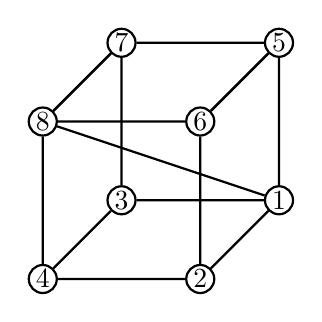
\begin{tikzpicture}[
roundnode/.style={circle, draw=black, thick, minimum size=2mm,inner sep= 0.25mm},
squarednode/.style={rectangle, draw=red!60, fill=red!5, very thick, minimum size=5mm},
]
    \node[roundnode]   (v1)   at   (1,1) {$1$};%   {\footnotesize $v_1$};
    \node[roundnode]   (v2)   at   (0,0) {$2$};%   {\footnotesize $v_1$};
    \node[roundnode]   (v3)   at   (-1,1) {$3$};%   {\footnotesize $v_1$};
    \node[roundnode]   (v4)   at   (-2,0) {$4$};%   {\footnotesize $v_1$};
    \node[roundnode]   (v5)   at   (1,3) {$5$};%   {\footnotesize $v_1$};
    \node[roundnode]   (v6)   at   (0,2) {$6$};%   {\footnotesize $v_1$};
    \node[roundnode]   (v7)   at   (-1,3) {$7$};%   {\footnotesize $v_1$};
    \node[roundnode]   (v8)   at   (-2,2) {$8$};%   {\footnotesize $v_1$};
    \draw[-,thick] (v1)--(v2)--(v4)--(v3)--(v1);
    \draw[-,thick] (v5)--(v6)--(v8)--(v7)--(v5);
    \draw[-,thick] (v1)--(v5)--(v6)--(v2);
    \draw[-,thick] (v3)--(v7)--(v8)--(v4);
    \draw[-,thick] (v1)--(v8);
    %\draw[-,thick] (v1)--(v4);
    %\draw[-,thick] (v1)--(v3);

\end{tikzpicture} \label{rigid example}
}
\qquad
\subfloat[]{ %{\resizebox{3cm}{!}
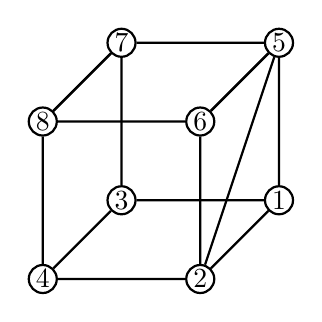
\begin{tikzpicture}[
roundnode/.style={circle, draw=black, thick, minimum size=2mm,inner sep= 0.25mm},
squarednode/.style={rectangle, draw=red!60, fill=red!5, very thick, minimum size=5mm},
]
    \node[roundnode]   (v1)   at   (1,1) {$1$};%   {\footnotesize $v_1$};
    \node[roundnode]   (v2)   at   (0,0) {$2$};%   {\footnotesize $v_1$};
    \node[roundnode]   (v3)   at   (-1,1) {$3$};%   {\footnotesize $v_1$};
    \node[roundnode]   (v4)   at   (-2,0) {$4$};%   {\footnotesize $v_1$};
    \node[roundnode]   (v5)   at   (1,3) {$5$};%   {\footnotesize $v_1$};
    \node[roundnode]   (v6)   at   (0,2) {$6$};%   {\footnotesize $v_1$};
    \node[roundnode]   (v7)   at   (-1,3) {$7$};%   {\footnotesize $v_1$};
    \node[roundnode]   (v8)   at   (-2,2) {$8$};%   {\footnotesize $v_1$};
    \draw[-,thick] (v1)--(v2)--(v4)--(v3)--(v1);
    \draw[-,thick] (v5)--(v6)--(v8)--(v7)--(v5);
    \draw[-,thick] (v1)--(v5)--(v6)--(v2);
    \draw[-,thick] (v3)--(v7)--(v8)--(v4);
    \draw[-,thick] (v2)--(v5);
\end{tikzpicture}
\label{norigid example}}
%    \subfloat[Non-infinitesimally bearing rigid framework.]{\includegraphics[width=0.45\columnwidth]{norigid.png}\label{norigid example}}\\
    \caption{Examples of infinitesimally/non-infinitesimally bearing rigid frameworks in three-dimensional space. %\textcolor{blue}{need new illustration}
    }
\end{figure}

An example of infinitesimally/non-infinitesimally bearing rigid frameworks in the two-dimensional space is depicted in Fig.~\ref{rigid example}-\ref{norigid example}. 
Suppose that there are $n_a$ agents ($0\leq n_a \leq n$), known as beacons, can measure their own real positions. The rest $n_f=n-n_a$ agents are
called followers (Note that the network cannot be localized without beacons). Without loss of generality, we denote the first $n_a$ agents as beacons ($V_a = \left\{1,2,...,n_a\right\}$) and the rest as followers ($V_f = \left\{n_a+1,n_a+2,...,n\right\}$). The bearing-based network localization problem can be stated as follows.

\textbf{Problem.} \emph{Assuming  framework $\mathcal{G}(\overline{\mathbf{x}})$ is infinitesimally bearing rigid and suppose that there exist at least $2\leq n_a< n$ beacon nodes which know their absolute positions. The initial position estimation of the system is $\hat{\overline{x}}(0)$. Design the update law for each agent $u_i(k)=\hat{\overline{x}}(k+1)-\hat{\overline{x}}(k)$ $\forall i \in V$ based on the relative estimates $\left\{\hat{\overline{x}}_i(k)-\hat{\overline{x}}_j(k)\right\}$ and the constant bearing measurements $\left\{g_{ij}\right\}$ such that $\hat{\overline{\mathbf{x}}}(k)\rightarrow \overline{\mathbf{x}}$ as $k\rightarrow \infty$ for all $i\in V$.} 

\subsection{Randomized bearing-based network localization}
Consider a network consisting of $n$ sensors (agents). %Each follower $i\in V$ stores its own estimation vector $\overline{x}_i \in \mathbb{R}^d$. 
%The randomized manner is specified by a random process $\gamma(k)\in V$ where $k\in \mathbb{Z}_{+}$ is called a time slot. 
At time slot $k$, %$\gamma(k) = i$ %(with probability $\frac{1}{n}$) 
%indicates 
suppose that agent $i$ wakes up, then it will choose another neighbor $j$ with a probability ${\rm P}_{ij}$ to communicate. If both the waken and chosen ones are beacons, then they just retain their values. If both the waken and chosen ones are followers, they will update their values simultaneously. If one of the two agents is a beacon and the other is a follower, only the follower can update its value. In summary, the updating law is designed as follows 

\begin{enumerate}
\item if $i$ and $j$ are beacons:
\begin{equation}\label{algorithmNL0}
    \begin{aligned}
    \overline{x}_i(k+1)&=\overline{x}_i(k)=x_i,\\
    \overline{x}_j(k+1)&=\overline{x}_j(k)=x_j.
    %W_{ij} &= \mathbf{I}_{dn\times dn}
    \end{aligned}
\end{equation}

\item if $i$ and $j$ are followers:
\begin{equation}\label{algorithmNL1}
    \begin{aligned}
    \hat{\overline{x}}_i(k+1)&=\hat{\overline{x}}_i(k)-\alpha \mathbf{A}_{ij}\big(\hat{\overline{x}}_i(k)-\hat{\overline{x}}_j(k)\big),\\
    \hat{\overline{x}}_j(k+1)&=\hat{\overline{x}}_j(k)-\alpha \mathbf{A}_{ji}\big(\hat{\overline{x}}_j(k)-\hat{\overline{x}}_i(k)\big).\\
    \end{aligned}
\end{equation}
\item if one of the partners is a beacon and the other is a follower (without loss of generality, assume $i$ is a follower)
\begin{equation}\label{algorithmNL2}
    \begin{aligned}
    \hat{\overline{x}}_i(k+1)&=\hat{\overline{x}}_i(k)-\alpha \mathbf{A}_{ij}\big(\hat{\overline{x}}_i(k)-\overline{x}_j(k)\big),\\
    \overline{x}_j(k+1)&=\overline{x}_j(k)=\overline{x}_j,
    \end{aligned}
\end{equation}
\end{enumerate}
where $\alpha > 0$ is updating step size.

% \begin{figure*}
% {\small 
%     \begin{equation} \label{eq:13}
% W_{ij}=\begin{bmatrix}
%     &\mathbf{I}_d        &\cdots     &\mathbf{0}             &\cdots    &\mathbf{0} &\cdots &\mathbf{0} \\
%     &\vdots     &\ddots     &\vdots          &\ddots    &\vdots &\ddots &\vdots \\
%     &\mathbf{0}        &\cdots  &\mathbf{I}_d-\alpha \mathbf{A}_{ij} &\cdots    &\alpha \mathbf{A}_{ij} &\cdots &\mathbf{0}  \\
%     &\vdots     &\ddots     &\vdots          &\ddots    &\vdots &\ddots &\vdots \\
%     &\mathbf{0}        &\cdots  &\alpha \mathbf{A}_{ji} &\cdots    &\mathbf{I}_d-\alpha\mathbf{A}_{ji} &\cdots &\mathbf{0}  \\
%     &\vdots     &\ddots     &\vdots          &\ddots    &\vdots &\ddots &\vdots \\
%     &\mathbf{0}        &\cdots     &\mathbf{0}             &\cdots    &\mathbf{0} &\cdots &\mathbf{I}_d
% \end{bmatrix}.
% \end{equation}}
% \end{figure*}

Denote $\Tilde{\overline{x}}_i(k)=\hat{\overline{x}}_i(k)-\overline{x}_i$ $\forall i \in V_f$ and $\Tilde{\overline{\mathbf{x}}} _f=[\Tilde{\overline{x}}_{n_a+1}^{\top},\Tilde{\overline{x}}_{n_a+2}^{\top},...,\Tilde{\overline{x}}_{n}^{\top}]^{\top}$. We subtract both sides of (\ref{algorithmNL1}) and (\ref{algorithmNL2}) by $p_f$. In addition, due to the fact that $\overline{x}_i-\overline{x}_j \in \text{null} (\mathbf{A}_{ij})$, a quantity $\alpha\mathbf{A}_{ij}(\overline{x}_i-\overline{x}_j)$ is added to the right-hand side of every follower's equation of (\ref{algorithmNL1}) and (\ref{algorithmNL2}). Thus, we can rewrite (\ref{algorithmNL0}-\ref{algorithmNL2}) as
\begin{equation}
\Tilde{\overline{\mathbf{x}}}_f =W_{ij}\Tilde{\overline{\mathbf{x}}}_f (k)
\end{equation}
where $W_{ij} \in \mathbb{R}^{n_fd\times n_fd}$ and can be determined as
\begin{enumerate}
\item if $i$ and $j$ are beacons:
\begin{equation}\label{algorithm01}
    \begin{aligned}
%    {p}_i(k+1)&={p}_i(k)\\
%    {p}_j(k+1)&={p}_j(k)\\
    W_{ij} &= \mathbf{I}_{dn\times dn}.
    \end{aligned}
\end{equation}

\item if $i$ and $j$ are followers, the updating matrix $W_{ij}$ is as given in \eqref{algorithm12}, with $\alpha_i=\alpha_j=\alpha$. %, where $\mathbf{0}$ denotes the $d\times d$ zero matrix, $\mathbf{I}_d-\alpha_i \mathbf{A}_{ij}$ is the block entry of matrix $W_{ij}$ in the $({i(d-1)+1:id})^{\text{th}}$ rows and $({i(d-1)+1:id})^{\text{th}}$ columns. Block $\mathbf{I}_d-~\alpha_j \mathbf{A}_{ij}$ is in the $({j(d-1)+1:jd})^{\text{th}}$ rows and $({j(d-1)+1:jd})^{\text{th}}$ columns of $W_{ij}$. 
\item if one agent $i$ is a follower and the other agent $j$ is a beacon, we have the updating matrix 
\begin{equation}\label{algorithm21}
\begin{aligned}
W_{ij} = \text{blkdiag}(\mathbf{I}_d,\dots,\mathbf{I}_d-\alpha \mathbf{A}_{ij},\dots,\mathbf{I}_d).
\end{aligned}
\end{equation}
\end{enumerate}
It can be seen that for all three scenarios, $W_{ij}$ is symmetric due to the symmetry of $\mathbf{A}_{ij}$. At a random $k^{\text{th}}$ time slot, we now can write
\begin{equation}\label{algorithmNL13}
\Tilde{\overline{\mathbf{x}}}_f (k+1)=W(k)\Tilde{\overline{\mathbf{x}}}_f(k),
\end{equation}
where the random variable $W(k)$ is drawn i.i.d from some distribution on the set of all possible $W_{ij}$. %Furthermore, since $\Tilde{{\overline{\mathbf{x}}}} _a(k)=\hat{{\overline{\mathbf{x}}}} _a(k)-{\overline{\mathbf{x}}} _a=\mathbf{0}$, the dynamic of the estimation errors of followers can be obtained as

%\begin{equation}\label{algorithmNL131}
%%\Tilde{\overline{\mathbf{x}}}_f (k+1)=W(k)\Tilde{\overline{\mathbf{x}}}_f (k),
%\end{equation}
%where $W$ is the block entry of $W(k)$ in the last $n_fd$ rows and $n_fd$ columns.

\begin{assume}\label{probability}
For every $(i,j)\in E$, ${\rm P}_{ij}+{\rm P}_{ji}>0$.   
\end{assume}
Note that $\mathbf{M}_{ij}=\frac{1}{n}(\mathbf{A}_{ij} {\rm P}_{ij}+\mathbf{A}_{ji} {\rm P}_{ji})=\frac{1}{n}({\rm P}_{ij}+{\rm P}_{ji})\mathbf{A}_{ji}$. Thus, Assumption~\ref{probability} implies that $\mathbf{M}_{ij}$ is positive semi-definite if and only if $\mathbf{A}_{ij}$ is positive semi-definite.
%It can be seen that the probability that two agents $i$ and $j$ communicate with each other is $\frac{1}{n}({\rm P}_{ij}+{\rm P}_{ji})$ (the probability that agent $i$ will wake up at $k^{\text{th}}$ time slot is $\frac{1}{n}$, and the probability that $j$ will be chosen by $i$ is ${\rm P}_{ij}$). 
The corresponding expected Laplacian matrix can be partitioned into the following form 
$$\mathbf{L}^{\rm M}(\mathcal{G})=\begin{bmatrix}
\mathbf{L}^{\rm M}_{aa} &\mathbf{L}^{\rm M}_{af} \\
\mathbf{L}^{\rm M}_{fa} &\mathbf{L}^{\rm M}_{ff} \\
\end{bmatrix},$$
where $\mathbf{L}_{aa}^{\rm M}$ is the block entry of matrix $\mathbf{L}^{\rm M}$ in the first $n_ad$ rows
and $n_ad$ columns.

\begin{lemma}
\text{\emph{\cite{bearingzhao}}}
 Suppose that $\mathcal{G}(\bar{\mathbf{x}})$ is infinitesimal bearing rigid, the matrix $\mathbf{L}^{\rm M}_{ff}$ is positive definite if and only if $n_a \geq 2$.
\end{lemma}

\begin{theorem}\label{NLmaintheorem}
  Suppose that $\mathcal{G}(\overline{\mathbf{x}})$ is infinitesimal bearing rigid and $n_a \geq 2$. Selecting the updating step size such that $\alpha<\underset{i,j \in V_f}{\min}(\frac{1}{\max\| \mathbf{D}^{\rm M}_{i} \|},\frac{2}{{\max}||\mathbf{A}_{ij}||})$, the first and second moment of the system \eqref{algorithmNL13} converges to zero as $k\to \infty$, i.e., the estimated configuration ${\hat{\overline{\mathbf{x}}}}(k)$ converges to the actual configuration $\overline{\mathbf{x}}$ as $k \to \infty$ in probability. 
\end{theorem}

\emph{Proof:} See Appendix D.
%%%%%%%%%%%%%%%%%%%%%%%%%%%%%
\section{Numerical examples}
\label{section: simulation}
\subsection{Randomized matrix weighted consensus  with Leaderless topology}
Consider a system of four agents whose state vectors are defined in $\mathbb{R}^3$. The matrix-weights of the system are given as
{\small
\begin{align*}
\mathbf{A}_{12}&= 
\begin{bmatrix}
1 &0 &0\\
0 &\frac{1}{2} &\frac{1}{5}\\
0 &\frac{1}{2} &1
\end{bmatrix},
\mathbf{A}_{21}= 
\begin{bmatrix}
4 &2 &0\\
2 &\frac{1}{2} &0\\
0 &0 &0
\end{bmatrix}, 
\mathbf{A}_{13}= 
\begin{bmatrix}
5 &\frac{1}{3} &0\\
\frac{1}{3} &\frac{1}{2} &0\\
0 &0 &0
\end{bmatrix},\\
\mathbf{A}_{31}&= 
\begin{bmatrix}
5 &\frac{1}{3} &0\\
\frac{1}{3} &\frac{1}{2} &0\\
0 &0 &1
\end{bmatrix},
\mathbf{A}_{23} = 
\begin{bmatrix}
1 &\frac{1}{2} &0\\
\frac{1}{2} &1 &0\\
0 &0 &\frac{1}{3}
\end{bmatrix},
\mathbf{A}_{32}= 
\begin{bmatrix}
1 &\frac{1}{2} &0\\
\frac{1}{2} &\frac{1}{2} &0\\
0 &0 &\frac{1}{3}
\end{bmatrix},\\
\mathbf{A}_{34} &= 
\begin{bmatrix}
2 &0 &\frac{1}{2}\\
0 &2 &0\\
\frac{1}{2} &0 &1
\end{bmatrix},
\mathbf{A}_{43}= 
\begin{bmatrix}
3 &0 &0\\
0 &1 &1\\
0 &1 &1
\end{bmatrix}.
\end{align*}
}
and zero matrices otherwise. The transition matrix $\pi = [{\rm P}_{ij}]$ is designed as follow
{
\begin{equation*}
\pi =  
\begin{bmatrix}
0 &\frac{1}{2} &\frac{1}{2} &0\\
\frac{1}{3} &0 &\frac{2}{3} &0\\
\frac{1}{2} &\frac{1}{4} &0 &\frac{1}{4}\\
0 &0 &1 &0
\end{bmatrix}.
\end{equation*}}
The initial vectors of the agents are given as $\overline{x}_1(0)=[1,-2,3]^\top, \overline{x}_2(0)=[0,6,3]^\top,\overline{x}_3(0)=[-1,10,1]^\top,\overline{x}_1(0)=[0,2,5]^\top$. The average state vector is thus $\hat{\overline{x}}=[0,4,3]^\top$. To meet Theorem \ref{upperbound1}, the agents' common step size is set at $\alpha=0.02$. As shown in Fig.~\ref{leaderless}, four agents achieve a consensus. Their convergence value is $[0.0,4.0,3.0]^\top$, which is the average.
\begin{figure}
\begin{center}
\includegraphics[height=6cm]{gossip_leaderless}    % The printed column  
\caption{Randomized matrix weighted consensus of four agents with
Leaderless topology}  % width is 8.4 cm.
\label{leaderless}                                 % Size the figures 
\end{center}                                 % accordingly.
\end{figure}
\subsection{Randomized MWC with Leader-Following topology}
We added a leader node $\overline{x}_0=[-1,3,1]^\top$ to the previous system. The leader-follower matrix-weights are given as { $ \mathbf{A}_{10}=
\begin{bmatrix}
1 & 0 & 0\\
0 & 1 & 0\\
0 & 0 & 0
\end{bmatrix},
\mathbf{A}_{20}=
\begin{bmatrix}
0 & 0 & 0\\
0 & 0 & 0\\
0 & 0 & 5
\end{bmatrix}
$} 
and zero matrices, otherwise. The common step size is set at $\alpha = 0.1, \theta=0.5$. The simulation result is depicted in Fig.~\ref{leader}. All agents asymptotically reach a consensus at leader's state vector $[-1,~3,~1]^\top$.
\begin{figure}
\begin{center}
\includegraphics[height=6cm]{gossip_leader}    % The printed column  
\caption{Randomized MWC of 5 agents with
Leader-Follower topology}  % width is 8.4 cm.
\label{leader}                                 % Size the figures 
\end{center}                                 % accordingly.
\end{figure}

\subsection{Randomized bearing-based network localization}\label{NL}

Consider a network of $n=62$ sensor nodes in a three-dimensional space ($d=3$), with $\overline{x}_i=[x_i,y_i,z_i]^{\top}$. There are $n_a=4$ beacons (nodes 1 to 4) in the network. As depicted in Fig.~\ref{trueConfig}, the sensor nodes are distributed around a sphere of radius 1.

The initial estimate $\hat{\overline{x}}_i(0)=[\hat{x}_i(0),\hat{y}_i(0),\hat{z}_i(0)]^\top$ of each follower node is generated randomly in a cubic $[-1.5,1.5]\times[-1.5,1.5]\times[-1.5,1.5]$, which is shown in Fig. \ref{est0}. The edges in $E$, being chosen accordingly to the proximity-rule
\[(i,j) \in E \Longleftrightarrow \|\bar{x}_i - \bar{x}_j\|\leq 0.75,\]
results to the topological graph $G$ in Fig.~\ref{trueConfig}.

The simulation result of the sensor network under the randomized network localization protocol \eqref{algorithmNL0}, \eqref{algorithmNL1}, \eqref{algorithmNL2} is illustrated in Fig.~\ref{fig:simNL}. As can be shown in Fig.~\ref{est0}--\ref{est1000}, the estimate configuration $\hat{\overline{x}}(k)$ at time instances $k=0, 100, 300, 500, 1000$, demonstrates that all position estimates eventually converge to the true value as $k$ increases. 

Additionally, it can be seen from Fig.~\ref{Berror} that the total bearing error, which is defined as $\sum_{(i,j)\in E} \|\mathbf{A}_{ij}(\hat{\overline{x}}_j(k)-\hat{\overline{x}}_i(k))\|^2$, converges to 0. Thus, the simulation result is consistent with the theoretical results. %An animation of the simulation can be found at {\url{https://youtube.com/shorts/5Xu05w2P8nM}}.
\begin{figure*}[ht]
    \centering
    \begin{minipage}{0.7\linewidth} 
    \subfloat[The network $\mathcal{G}(\mathbf{x})$.]{\includegraphics[width=0.33\textwidth]{trueNetwork.png} \label{trueConfig}} \hfill
    \subfloat[$\hat{\overline{x}}(0)$.]{\includegraphics[width=0.33\textwidth]{network_N_0}\label{est0}}\hfill
    \subfloat[$\hat{\overline{x}}(100)$]{\includegraphics[width=0.33\textwidth]{network_N_100.png}\label{est100}} \hfill
    \subfloat[$\hat{\overline{x}}(300)$]{\includegraphics[width=0.33\textwidth]{network_N_300.png}\label{est300}} \hfill
    \subfloat[$\hat{\overline{x}}(500)$]{\includegraphics[width=0.33\textwidth]{network_N_500.png}\label{est500}}\hfill
    \subfloat[$\hat{\overline{x}}(1000)$]{\includegraphics[width=0.33\textwidth]{network_N_1000.png}\label{est1000}}
    \end{minipage}%
    \hfill
    \begin{minipage}{0.3\linewidth}
    \centering
    \subfloat[Bearing error vs time.]{\includegraphics[width=0.88\textwidth]{err.png}\label{Berror}}
    \end{minipage}%
    \caption{Simulation of a sensor network consisting of 62 nodes under the gossip-based network localization protocol \eqref{algorithmNL0}, \eqref{algorithmNL1}, \eqref{algorithmNL2}: (a) - the network $\mathcal{G}(\bar{\mathbf{x})}$ (beacon nodes are denoted with `$\textcolor{blue}{\boldsymbol{\Delta}}$', normal nodes are denoted by `\textbf{o}', respectively); From (b) to (f) - the estimate configurations at different time instances; (g) the bearing error vs time. \label{fig:simNL}} 
\end{figure*}

\section{Conclusion}\label{sec:conclusion}
In this paper, two randomized matrix-weighted consensus algorithms for both leaderless and leader-following topologies have been developed. We started with the general protocol, in which agents update their vector state in a randomized asynchronous manner. It was shown that, under some mild assumptions and by choosing a small enough updating step size, the agents could reach consensus in expectations. Furthermore, the upper bound of the convergence rate could be predetermined given the knowledge of each agent's probability distribution. The proposed framework is then applied to a bearing-based network localization problem. Finally, numerical examples verified the theoretical result. One of our future research directions is to apply optimization techniques to find the optimal probability distribution for each agent, which will improve the consensus speed of the system.

% \section*{Acknowledgments}
% \textcolor{blue}{To access the full version of Section~\ref{NL}, we refer readers to our arXiv paper \cite{arxiv}.}

 % argument is your BibTeX string definitions and bibliography database(s)
%\bibliography{IEEEabrv,../bib/paper}
%
\section*{Appendix}
%\appendix
%\section{Proof of Lemma \ref{stepsizeav}}    % Each appendix must have a short title.

\subsection{Proof of Lemma \ref{stepsizeav}}
$\bullet$ \emph{The set of all real symmetric matrices with eigenvalues in $[0,1]$ is convex. Every possible matrix $W_{ij}^\top W_{ij}$ is in this set.}

The first part of this statement is a consequence of the following lemma \cite{Rajendramatrix2}: \emph{A, B are n×n Hermitian matrices. If the eigenvalues of A and B are all in an interval I, then the eigenvalues of any convex combination of A and B are also in I.} 

Rearrange the rows and columns of $W_{ij}$ we get
{
\begin{equation}
W_{ij}=\begin{bmatrix}
        &\mathbf{I}_d-\alpha_i \mathbf{A}_{ij} &\alpha_i \mathbf{A}_{ij} &\cdots &\mathbf{0}  \\
        &\alpha_j \mathbf{A}_{ij} &\mathbf{I}_d-\alpha_j\mathbf{A}_{ij} &\cdots &\mathbf{0}  \\
       &\vdots          &\vdots    &\ddots  &\vdots \\
        &\mathbf{0}   &\mathbf{0}    &\cdots &\mathbf{I}_d  \\
\end{bmatrix}.
\end{equation}}
Thus, the union of the unity eigenvalues (which correspond to the identity matrices $\mathbf{I}_d$) and the eigenvalues of matrix $w=
\begin{bmatrix}
    &\mathbf{I}_d-\alpha_i \mathbf{A}_{ij} &\alpha_i \mathbf{A}_{ij}\\
    &\alpha_j \mathbf{A}_{ij} &\mathbf{I}_d-\alpha_j\mathbf{A}_{ij} \\
\end{bmatrix}
$ yields the eigenvalues of $W_{ij}$. By choosing $\alpha<\frac{1}{\max\lVert \mathbf{A}_{ij} \rVert}$, we can easily obtain $-1<\lambda(w)\leq 1$ (see Lemma \ref{stepsize}). $W_{ij}$'s eigenvalues then satisfy $\lambda(W_{ij}) \in (-1,1]$. Hence, $\lambda(W_{ij}^{\top}W_{ij})=\lambda(W_{ij}^2)=\lambda(W_{ij})^2 ~\in [0,1]$.

$\bullet$ \emph{${\rm E}[W(k)^\top W(k)]$ has a unity spectral radius, and its unity eigenvalues are semi-simple.}

We take into account ${\rm E}[W(k)^{\top}W(k)]$  as a convex combination of all possible $W_{ij}^2$. As a result, using the first statement of Lemma \ref{stepsizeav}, ${\rm E}[W(k)^\top W(k)]$ has a unity spectral radius. Due to the symmetry of ${\rm E}[W(k)^{\top}W(k)]$,
its unity eigenvalues are semi-simple.

$\bullet$ \emph{$\mathbf{1}_n \otimes\mathbf{I}_d$ are 
only $d$ orthogonal right eigenvectors corresponding to the unity eigenvalues $\lambda=1$ of ${\rm E}[W(k)^\top W(k)]$ if and only if null$(\mathbf{L}^{\rm M})=\text{range}(\mathbf{1}_n\otimes \mathbf{I}_d)$}.

Using (\ref{algorithm12}), we can easily get the following:
{\small
\begin{equation*}
W_{ij}^{\top}W_{ij}=\begin{bmatrix}
    &\mathbf{I}_d        &\cdots     &\mathbf{0}             &\cdots    &\mathbf{0} &\cdots &\mathbf{0} \\
    &\vdots     &\ddots     &\vdots          &\ddots    &\vdots &\ddots &\vdots \\
    &\mathbf{0}        &\cdots  &\mathbf{I}_d-\mathbf{\hat{A}}_{ij} &\cdots    &\mathbf{\hat{A}}_{ij} &\cdots &\mathbf{0}  \\
    &\vdots     &\ddots     &\vdots          &\ddots    &\vdots &\ddots &\vdots \\
    &\mathbf{0}        &\cdots  &\mathbf{\hat{A}}_{ij} &\cdots    &\mathbf{I}_d-\mathbf{\hat{A}}_{ij} &\cdots &\mathbf{0}  \\
    &\vdots     &\ddots     &\vdots          &\ddots    &\vdots &\ddots &\vdots \\
    &\mathbf{0}        &\cdots     &\mathbf{0}             &\cdots    &\mathbf{0} &\cdots &\mathbf{I}_d 
\end{bmatrix}
\end{equation*}}
where $\mathbf{\hat{A}}_{ij}=2\alpha \mathbf{A}_{ij}(\mathbf{I}_d-\alpha \mathbf{A}_{ij})$. Denote $\mathbf{\hat{M}}_{ij}= \frac{1}{n}(\mathbf{\hat{A}}_{ij} {\rm P}_{ij}+\mathbf{\hat{A}}_{ji} {\rm P}_{ji})$. By choosing $0<\alpha<\frac{1}{\max\lVert \mathbf{A}_{ij} \rVert}$, $\mathbf{\hat{A}}_{ij}$ is positive definite (resp., positive semi-definite) if and only if $\mathbf{A}_{ij}$ is positive definite (resp., positive semi-definite). The same kind of relationship also holds for $\mathbf{\hat{M}}_{ij}$ and $\mathbf{M}_{ij}$. Moreover, it is simply provable that $\text{null}(\mathbf{\hat{A}}_{ij})=\text{null}(\mathbf{A}_{ij})$ and thus $\text{null}(\mathbf{\hat{M}}_{ij})=\text{null}(\mathbf{M}_{ij})$. We now rewrite ${\rm E}[W(k)^\top W(k)]$ as 
$${\rm E}[W(k)^\top W(k)]=\mathbf{I}_{dn} - (\mathbf{\hat{D}}^{\text{M}}-\mathbf{\hat{A}}^\text{M})=\mathbf{I}_{dn} - \mathbf{\hat{L}}^\text{M},$$
in which $\mathbf{\hat{D}}^{\text{M}}= \text{blkdiag}(\mathbf{\hat{D}}^{\text{M}}_{1},\ldots,\mathbf{\hat{D}}^{\text{M}}_{n})$, whereas $\mathbf{\hat{D}}^{\text{M}}_{i}= \sum_{j \in V}\mathbf{\hat{M}}_{ij}$ and $\mathbf{\hat{A}}^\text{M}=[\mathbf{\hat{M}}_{ij}]$. It is clear that the eigenvectors corresponding to the unity eigenvalue of ${\rm E}[W(k)^\top W(k)]$ is the null space of $\mathbf{\hat{L}}^\text{M}$. Similar to Lemma \ref{nullspace}, the following holds:
  $\text{null}(\mathbf{\hat{L}}^{\text{M}}) =  \text{span}\{ \text{range}(\mathbf{1}_n \otimes \mathbf{I}_d),  \{ \mathbf{v}=[v_1^\top,\dots, v_n^\top]^\top \in \mathbb{R}^{nd}|~(v_j-v_j)\in \text{null}(\mathbf{\hat{M}}_{ij})=\text{null}(\mathbf{M}_{ij}), \forall (i,j) \in V \} \}$. Therefore, $\text{null}(\mathbf{\hat{L}}^{\text{M}})=\text{range}(\mathbf{1}_n\otimes \mathbf{I}_d)$ if and only if $\text{null}(\mathbf{L}^{\text{M}})=\text{range}(\mathbf{1}_n\otimes \mathbf{I}_d)$.
 
\subsection{Proof of Theorem \ref{ddmwc}}
Denote the error vector $\overline{y}_i(k)=\overline{x}_i(k)-\overline{x}_0$. System (\ref{algorithm2}) can be rewritten as
\begin{equation}\label{B1}
    \begin{aligned}
    \overline{y}_i(k+1)&=\overline{y}_i(k)- \theta\alpha\sum_{j\in \mathcal{N}_i} \mathbf{A}_{ij}\big(\overline{y}_i(k)-\overline{y}_j(k)\big)\\
    &\quad- (1-\theta)\alpha \mathbf{A}_{i0} \overline{y}_i(k).
    \end{aligned}
\end{equation}
For the whole system, (\ref{B1}) becomes
\begin{align} \label{B2}
    \mathbf{\overline{y}}(k+1)&=\big(\mathbf{I}_{dn}-\theta\alpha \mathbf{L}-(1-\theta)\alpha \text{blkdiag}({\mathbf{A}_{i0}})\big)\mathbf{\overline{y}}(k) \nonumber\\
    &=(\mathbf{I}_{dn}-\mathbf{N})\mathbf{\overline{y}}(k) =\mathbf{H}\mathbf{\overline{y}}(k),
\end{align}
where $\mathbf{\overline{y}}(k)=\text{vec}(\overline{y}_i(k))$.  

Choosing the updating step sizes $\alpha$ satisfy Theorem \ref{ddmwc}, we have $\lambda(\alpha\mathbf{L})$, $\lambda(\alpha\text{blkdiag}({\mathbf{A}_{i0}})) \in [0,2) $ and thus the convex combination of these two matrices $\mathbf{N}$ satisfy $0\leq\lambda(\mathbf{N})<2$ and $-1<\lambda(\mathbf{H})\leq1$.
Under the assumptions (\ref{Ai0}) and (\ref{nullL}), $\mathbf{N}$ is positive definite (the complete proof can be found in \cite{Nguyen2022MCA}) and then $\lambda(\mathbf{H})<1$. As a result, it yields $-1<\lambda(\mathbf{H})<1$. 
The matrix $\mathbf{H}$ is thus stable, and $\mathbf{\overline{y}}(k)\rightarrow 0$ as $k \rightarrow \infty$. Furthermore, it is well known from linear control theory that the converge rate of $\mathbf{\overline{y}}(k)$ will depend on the largest-in-magnitude eigenvalue of $\mathbf{H}$.

  
\subsection{Proof of Theorem \ref{2mmlf}}
Choosing the updating step sizes $\alpha$ satisfy Theorem \ref{2mmlf}, it is easily obtained that each possible $W_{ij}$ has eigenvalues satisfy $-1<\lambda(W_{ij})\leq 1$ and thus $0\leq\lambda(W_{ij}^\top W_{ij})\leq 1$. Denote $\left\{v_{ij}\right\}$ as the eigenspace of $W_{ij}$ corresponding to the eigenvalue $\lambda=1$. Clearly, $\left\{v_{ij}\right\}$ is also the eigenspace corresponding to the unity eigenvalue of $W_{ij}^\top W_{ij}$. We now treat the expectation ${\rm E}[W_{ij}]$ (resp., ${\rm E}[W_{ij}^\top W_{ij}]$)  as a convex combination of all possible $W_{ij}$ (resp., $W_{ij}^\top W_{ij}$) where ${\rm P}_{ij}\neq 0$. Because $W_{ij}$ is symmetric (and thus $W_{ij}^\top W_{ij}$), ${\rm E}[W_{ij}]$ cannot have a unity eigenvalue unless there exists a common eigenvector between every eigenspace $\left\{v_{ij}\right\}$. From Theorem \ref{ddmwc}, we already have $-1<\lambda({\rm E}[W_{ij}])<1$, which implies $\underset{{\rm P}_{ij}\neq 0}{\bigcap}\left\{v_{ij}\right\}=\varnothing$. Thus, it is obvious that $0\leq \lambda({\rm E}[W_{ij}^\top W_{ij}])<1$. This completes the proof of Theorem \ref{2mmlf}.


\subsection{Proof of Theorem \ref{NLmaintheorem}}
The proof is divided into two parts:

$\bullet$ \emph{Convergence in Expectation.} Taking the expectation of \eqref{algorithmNL13} yields ${\rm E}[W(k)]=\mathbf{I}_{n_f}-\alpha\mathbf{L}^{\rm M}_{ff}$, 
which implies that
\begin{equation}\label{expcet}
    \begin{aligned}
       % \hat{p}_a(k+1)&=\hat{p}_a(k)=p_a,\\
        {\rm E}[\Tilde{\overline{\mathbf{x}}} _f(k+1)]
        &=(\mathbf{I}_{n_f}-\alpha \mathbf{L}^{\rm M}_{ff}){\rm E}[\Tilde{\overline{\mathbf{x}}} _f(k)]\\
        &=(\mathbf{I}_{n_f}-\alpha \mathbf{L}^{\rm M}_{ff})^{k+1}\Tilde{\overline{\mathbf{x}}} _f(0).
    \end{aligned}
\end{equation}
Similar to Appendix B, it could be easily obtained that by choosing the stepsize $\alpha <\underset{i \in V_f}{\min}\frac{1}{\max\| \mathbf{D}^{\rm M}_{i} \|}$, the following holds $-1<\lambda(\mathbf{I}_{n_f}-\alpha \mathbf{L}^{\rm M}_{ff}))\leq1$. Noting that the matrix $\alpha \mathbf{L}^{\rm M}_{ff}$ has already been confirmed to be symmetric and positive definite. Hence, $-1<\lambda(\mathbf{I}_{n_f}-\alpha \mathbf{L}^{\rm M}_{ff}))<1$, i.e., system (\ref{expcet}) is exponentially stable. As a result, ${\rm E}[\Tilde{\overline{\mathbf{x}}} _f(k+1)]\rightarrow 0$ as $k\rightarrow \infty$.

$\bullet$ \emph{Convergence of the Second Moment.} From the previous results, we obtain the following equation
\begin{equation}\label{secondmomentNL}
    \begin{aligned}
        {\rm E}[\Tilde{\overline{\mathbf{x}}}_f(k+1)^{\top}&\Tilde{\overline{\mathbf{x}}}_f(k+1)|\Tilde{\overline{\mathbf{x}}}_f(k)] \\
        &= \Tilde{\overline{\mathbf{x}}}_f(k)^{\top}{\rm E}[W(k)^{\top}W(k)]\Tilde{\overline{\mathbf{x}}}_f(k).
    \end{aligned}
\end{equation}

Hence, the proof of this part is similar to that of Theorem~\ref{2mmlf}.  Additionally, it can be easily obtained that the upper bound of $\epsilon$-consensus time of the proposed algorithm is as follows
$$K(\epsilon)=\frac{3{\log}(\epsilon^{-1})}{{\log}\lambda_{max}^{-1} \big( {\rm E}[{W}(k)^\top {W}(k)] \big)}.$$

%By choosing the updating step sizes $\alpha$ to satisfy Theorem~\ref{NLmaintheorem}, it can be obtained that each possible value of $W(k)$ has eigenvalues that satisfy $-1<\lambda(W(k))\leq 1$ and thus $0\leq\lambda(W(k)^\top W(k))\leq 1$. Denote $\left\{v_{ij}\right\}$ as the eigenspace of $W_{ij}$ corresponding to the eigenvalue $\lambda=1$. Clearly, $\left\{v_{ij}\right\}$ is also the eigenspace corresponding to the unity eigenvalue of $W_{ij}^\top W_{ij}$. We now treat the expectation ${\rm E}[W_{ij}]$ (resp., ${\rm E}[W_{ij}^\top W_{ij}]$)  as a convex combination of all possible $W_{ij}$ (resp., $W_{ij}^\top W_{ij}$) where ${\rm P}_{ij}\neq 0$. Because $W_{ij}$ is symmetric (and thus $W_{ij}^\top W_{ij}$), ${\rm E}[W_{ij}]$ cannot have a unity eigenvalue unless there exists a common eigenvector between every eigenspace $\left\{v_{ij}\right\}$. From Theorem \ref{steady}, we already have $-1<\lambda({\rm E}[W_{ij}])<1$, which implies $\underset{{\rm P}_{ij}\neq 0}{\bigcap}\left\{v_{ij}\right\}=~\varnothing$. Thus, it is obvious that $0\leq \lambda({\rm E}[W_{ij}^\top W_{ij}])<1$. This completes the proof.


\bibliographystyle{IEEEtran}
%\newpage
\bibliography{ref}
%\begin{IEEEbiography}[]{Nhat-Minh Le-Phan} is a Research Engineer at Research and Development in Navigation, Guidance and Control
%technologies center, Viettel Aerospace Institute, Hanoi, Vietnam. He received the B.S. in Control and Automation Engineering (2022) from Hanoi University of Science and Technology (HUST), Hanoi, Vietnam. He is currently pursuing the M.S. degree in Control and Automation Engineering at HUST. His current research interests include control of network systems and stochastic control.
%\end{IEEEbiography}
%
%\begin{IEEEbiography}[]{Minh Hoang Trinh} was a lecturer at the Department of Automatic Control, School of Electrical Engineering, Hanoi University of Science and Technology (HUST), Hanoi, Vietnam. He received the B.S. degree (2013) in electrical engineering from HUST, the M.S. degree (2015) in mechatronics and the Ph.D. degree (2018) in mechanical engineering both from Gwangju Institute of Science and Technology (GIST), Gwangju, Korea. 
%
%In 2016, he was at Technion - Israel Institute of Technology, for a six-month research visit. Prior to joining HUST in May 2019, he served as a Postdoc researcher at GIST. His research interests include distributed control of multi-agent systems, graph rigidity theory.
%\end{IEEEbiography}
%
%\begin{IEEEbiography}[]{Phuoc Doan Nguyen} received the Dipl.-Ing. in Technical Cybernetic in 1981 and Dr.-Ing. in Steuerungs- und Regelungstheorie in 1994, all at Technische Universit\"{a}t Dresden, Germany. He is currently a Professor at the Department of Automatic Control, School of Electrical Engineering, Hanoi University of Science and Technology (HUST), Hanoi,  Vietnam.
%Before joining HUST in 1997, he had served several years as research engineer in VEB Robotron Germany, in Institute 481 for Nuclear Energy Vietnam. His research interests are in the theory of nonlinear control systems, robust and adaptive control, optimization and optimal control.
%\end{IEEEbiography}
% You can push biographies down or up by placing
% a \vfill before or after them. The appropriate
% use of \vfill depends on what kind of text is
% on the last page and whether or not the columns
% are being equalized.

%\vfill

% Can be used to pull up biographies so that the bottom of the last one
% is flush with the other column.
%\enlargethispage{-5in}



% that's all folks
\end{document}


